\chapter{Background} \label{chap:background}

% You should provide enough background to the reader 
% for them to understand what the project is all about, 
% and what is the relevant prior work.
% Examiners like to know that you have done the 
% appropriate background research and it is important 
% that you review either what has been done previously 
% to tackle related problems, or perhaps what other 
% products exist related to your deliverable. Clear 
% references are important here, and much of this 
% section will typically already have been written in your 
% Interim Report. You may use feedback from that 
% report to improve what you write in your Final Report, 
% and should note that self-plagiarism between the two 
% reports is not possible, so no citation is needed of 
% your own earlier writing.

%  What does the reader need to know in order 
% to understand the rest of the report? What 
% problem are you solving?
%  Why is this problem interesting or worthwhile 
% to solve?
%  Who cares if you solve it?
%  How does this relate to other work in this 
% area?
%  What work does it build on?
%  For 'research-style' projects involving the 
% design and analysis of specific algorithms 
% there is a large amount of relevant 
% background both of general theory, and very 
% specific to the algorithm you investigate. 
% Supervisors will help you to see what is most 
% important here, but the general rule is that 
% you must both provide overall context and 
% note work close to what you do that 
% influences your work or is in some way 
% comparable to your work.

This chapter outlines background information required for understanding the basis for the project. The theory and literature serves to outline the main concepts used for neuromorphic data processing, as well as to reveal gaps in existing research that require solidifying.

\section{Event Cameras}

Event based cameras can be described as `bio-inspired sensors that differ from conventional frame cameras: Instead of capturing images at a fixed rate, they asynchronously measure per-pixel brightness changes, and output a stream of events that encode the time, location and sign of the brightness changes' \cite{EventBasedVisionASurvery}.

\subsection{Benefits} \label{ssec:event_camera_benefits}
Event-based cameras are purported to provide a number of benefits including;

\begin{itemize}
      \item \textbf{High temporal resolution}

            The reason for this is that whereas frame-based cameras have a certain frame-rate, event-based cameras do not have this limitation, meaning the "blind time" between frames is eliminated. The reason for this is that the function of a frame-based camera is dependent on the global shutter to capture the light at a particular instant, whereas event-based cameras can be thought of as having individual shutters for each pixel that are shut whenever an event occurs.
      \item \textbf{High dynamic range}

            The reason for this is again the fact that each pixel has its own individual shutter, but as well as this they all use a logarithmic scale, meaning they function well from very bright to very dim environments as well as fast shifts between the two.
      \item \textbf{Low power consumption}
      \item \textbf{High pixel bandwidth}

            Each pixel can capture events at the rate of ~kHz. This has the effect of reducing blur since there is a very high temporal resolution to begin with. This makes the system very responsive and therefore ideal for real-time systems.
      \item \textbf{Efficient Encoding}

            Since events are asynchronous and spatially sparse (i.e there are mainly 0 values in the output matrix), the encoding is very efficient, as opposed to frame-based cameras that produce data that is very spatially dense.
\end{itemize}

The above benefits are very persuasive reasons to adopt neuromorphic cameras in many different applications. It is conceivable that if algorithms can make use of these benefits (since most classical algorithms play to the strengths of the data generated by frame-based cameras), real-time systems could be completely revolutionised.

\subsection{Function} \label{ssec:event_camera_function}
Event-based cameras differ from frame based cameras fundamentally, in that they do not rely on a global shutter closing at regular intervals to record information of a scene. Instead each pixel closes whenever it detects an `event' occurring. The way such events are detected is dictated by the `event generation model'\cite{EventBasedVisionASurvery}.

Each pixel responds to changes in its log photo-current ($ L = log(I) $, where $I$ is the perceived brightness), giving the system a very high dynamic range. A recorded event `$ k $' has the format $ e_k = (\boldsymbol{\mathbf{x}}_k, t_k, p_k ) $. This is known as the Address Event Representation (AER). The first value is the spacial location of the event ($ \boldsymbol{\mathbf{x}}_k = (x_k, y_k)^\top $), the second value $ t_k $ is the temporal location, and the final value $ p_k \in {1, -1} $ indicates the polarity of the event (i.e in which direction the brightness gradient was changing). The brightness increment between two events at the same pixel is given by the equation $ \Delta L(\boldsymbol{\mathbf{x}}_k, t_k) = L(\boldsymbol{\mathbf{x}}_k, t_k) - L(\boldsymbol{\mathbf{x}}_k, t_k - \Delta t_k) $. In a perfect (noise free) environment an event is fired whenever the brightness increment reaches a temporal contrast threshold. This relationship is shown in \cref{eq:ideal_event_equation}.

\begin{equation}
      \Delta L(\boldsymbol{\mathbf{x}}_k, t_k) = p_k C ( C > 0 )
      \label{eq:ideal_event_equation}
\end{equation}

It should be noted that the value of $ C $ could be variable and therefore different for $ p_k = \pm 1 $. Additionally, we can approximate the temporal derivative of a pixels brightness by substituting \cref{eq:ideal_event_equation} into the Taylor expansion given in \cref{eq:temporal_derivative_taylor_exp}. \cref{eq:temporal_derivative} shows the resulting format for the temporal derivative.

\begin{equation}
      \Delta L(\boldsymbol{\mathbf{x}}_k, t_k) \approx \frac{\delta L}{\delta t}(\boldsymbol{\mathbf{x}}_k, t_k)\Delta t_k
      \label{eq:temporal_derivative_taylor_exp}
\end{equation}

\begin{equation}
      \frac{\delta L}{\delta t}(\boldsymbol{\mathbf{x}}_k, t_k) \approx \frac{\Delta L(\boldsymbol{\mathbf{x}}_k, t_k)}{\Delta t_k} = \frac{p_k C}{\Delta t_k}
      \label{eq:temporal_derivative}
\end{equation}

It should however be noted that the approximation in \cref{eq:temporal_derivative_taylor_exp} is only true under the assumption that $ \Delta t_k $ is exceedingly small. Since unlike frame-based cameras we do not measure absolute brightness, this is an indirect way of measuring and keeping track of the brightness within the frame.

\cref{fig:davis_camera} shows the basic functionality of an event-based camera. Shown in \textbf{(a)} is the simplified circuit diagram of the DAVIS pixel, which in \textbf{(b)} is used to convert light into events (shown in real life in images \textbf{(c)} and \textbf{(d)}). \textbf{(e)} shows how this setup would view a white square rotating on a black disk. It is a stream of events going from the past in green to the present in red. These events can then be seen overlaid on a natural scene in \textbf{(f)}.

\begin{figure}[htb]
      \centering
      \includegraphics[width=0.5\textwidth]{background/images/davis_camera.png}
      \caption{A summary of the functionality of the DAVIS event based camera\cite{EventBasedVisionASurvery}.}
      \label{fig:davis_camera}
\end{figure}

\section{Spiking Neural Networks and Neural Heterogeneity} \label{ssec:snn_and_heterogeneity}

\Cref{ssec:event_camera_benefits} lists some persuasive reasons for utilising neuromorphic systems, but there still many challenges posed when attempting to do so. For example, each pixel only responds to brightness change, but the problem is that such a change could be a result of not only scene changes, but also the position of the camera within the scene. For this reason most neuromorphic systems have currently been limited to stationary cameras. As well as this, the system is especially prone to stochastic noise due to inherent shot noise in photons and from transistor circuit noise \cite{EventBasedVisionASurvery}. For this reason \cref{eq:ideal_event_equation} can only be said to be true under ideal conditions. A more realistic model for events fired is a probabilistic event generation model. These take into consideration the aforementioned sources of noise. One such model is given by P. Lichtsteiner \textit{et al.}\cite{NonIdealEventCamera}, where sensor variation measurements suggested a normal distribution centred around $ C $ for event triggers.

In order to tackle issues such as the ones due to noise, it is useful to look at existing examples of spiking neural systems, such as a biological brain. It is known that the brain is heterogeneous on every scale, in the past this was thought to be simply a by-product of noisy processes, but more recently it can be shown that by adding heterogeneity to Spiking Neural Networks (SNNs), a more stable and robust system can be created\cite{NeuralHetroPromRobLearn}, indicating this heterogeneity has a more deep rooted purpose. As well as this the learned neural parameters tend to resemble what can observed experimentally. This may serve as an explanation for how the brain has evolved to deal with the many stochastic processing it encounters.

The foundations of SNNs are in computational neuroscience. The mechanisms of neurons in the brain are the inspiration behind creating ANNs with neurons that spike in the same way. Neurons in an a typical ANN have a weight, bias and activation function. This means that the output of the neurons can be summarised by \cref{eq:artificial_neuron_output}.

\begin{equation}
      y = \theta(\sum^n_{j=1}w_jx_j-u_j)
      \label{eq:artificial_neuron_output}
\end{equation}

This model was inspired by the biological neuron model shown in \cref{fig:biological_neuron}. The function of the neuron is similar in that it produces an output based on a function of the input stream, but the form of this output is in the form of a `spike' rather than a continuous function. The $ \Sigma $ shown in the diagram is actually the integration of all excitory and inhibitory input signals to the dendrites coming from the soma of the neuron. We can see that the electric potential of the neuron needs to exceed a certain threshold in order for the output of the neuron to be a spike. Spiking neural networks use a similar model of neurons in order to leverage the aforementioned benefits of neural heterogeneity.

\begin{figure}[htb]
      \centering
      \includegraphics[width=0.4\textwidth]{background/images/biological_neuron.png}
      \caption{A diagram of structure and function of a biological neuron \cite{BiologicalNeuronModel}.}
      \label{fig:biological_neuron}
\end{figure}

With SNNs it is theoretically possible to achieve very high energy efficiency, and when combined with a novel surrogate gradient and Recurrent Neural Network (RNN) as was experimented with in a paper by Bojian Yin \textit{et al.}\cite{EfficientSNN} excels in challenging tasks such as gesture recognition, and at some points even outperforms traditional ANNs. Alongside the aforementioned neural heterogeneity to combat stochastic processes we can see substantial improvements in previous SNN performance.

\section{Existing Algorithms for Event Analysis} \label{sec:existing_algorithms}

For SLAM, pose estimation and classification tasks the problem again is that classical systems heavily rely on the structure of conventional camera's outputs, and so there needs to be a radical paradigm shift in order to take events as inputs instead.

\subsection{Optic-flow Methods}

Since obtaining the equation for the temporal derivative in \cref{eq:temporal_derivative}, there is now a indirect measure of brightness and so a more classic computer vision techniques using optic-flow constraints can be utilised to characterise the events detected by pixels. In frame-based systems, optic flow methods create a flow-field that describe the displacement vector (signifying direction and magnitude of movement) for each pixel in the frame, and a similar derivation can be done for event data. A core constraint in this derivation is that the intensity of a local time-varying image region is constant under motion (for at least a short amount of time)\cite{GenerativeEventModel}. \cref{eq:optic_flow} is the resulting equations that shows the relation between the brightness gradient and the displacement of the pixel over a short period of time given its velocity\cite{EventBasedVisionASurvery}. It implies that if the motion is parallel to the edge, there is no event fired (since $ v \cdot \nabla L = 0  $) and conversely if the motion is perpendicular to the edge events are fired at their highest rate.

\color{red} TODO: Write about how optic flow is often used in classification to see in a frame what the directions of motion are as well as the frame itself and the laplacian or edge map. \color{black}

\begin{equation}
      \Delta L \approx -\nabla L \cdot v \Delta t_k
      \label{eq:optic_flow}
\end{equation}

\subsection{Frame Integration of Event Streams} \label{ssec:frame_integration}

A common method of getting frame-like videos from event data is to use the event-to-frame integration method. One such method is outlined by \textit{Wei Fang et al.}\cite{LearnableMembraneSNN}, which is the one used in the python package spikingjelly\cite{SpikingJelly}. The method used is outlined in \cref{eq:event_integration}.

Data in neuromorphic datasets are in the formulation of $ E(x_i, y_i, t_i, p_i) $ that represent the event's coordinate, time and polarity. We split the event's number $ N $ into $ T $ slices with nearly the same number of events in each slice and integrate events to frames. Note that $ T $ is also the simulating time-step. Denote a two channels frame as $ F(j) $ and a pixel at $ (p, x, y) $ as $ F(j, p, x, y) $, the pixel value is integrated from the events data whose indices are between $ j_l $ and $ j_r $:

\begin{align*}
      j_l = \lfloor \frac{N}{T} \rfloor \cdot j
\end{align*}
 
\begin{align*}
      j_r = \begin{cases}
            \lfloor \frac{N}{T} \rfloor \cdot (j + 1), & \text{if j < T - 1}\\
            N, & \text{if j = T - 1}\\
          \end{cases}
\end{align*}

\begin{equation}
      F(j, p, x, y) = \sum^{j_r -1}_{i=j_l}I_{p, x, y}(p_i, x_i, y_i)
      \label{eq:event_integration}
\end{equation}
 
where $ \lfloor . \rfloor $ is the floor operation, $ I_{p, x, y}(p_i, x_i, y_i) $ is an indicator function and it equals 1 only when $ (p, x, y) = (p_i, x_i, y_i) $.

\color{red} TODO: Write more about this method from the spikingjelly docs \color{black}

% \subsection{Localisation using Probabilistic Filters} \label{ssec:prob_filters}

% \subsubsection{Bayesian Inference}

% Unlike most other previous systems, probabilistic filters such as Bayesian filters are very much suited to work with data from event-based cameras. The reason for this is that it depends on iterative updates to the location probabilities using inputs, for which spiking inputs are ideal. Bayes's theorem can be derived from simple probabilistic rules\cite{BayesLaw}. We know $P(X|Y) = \frac{P(X, Y)}{P(Y)} $ and similarly $ P(Y|X) = \frac{P(Y, X)}{P(X)} $. Therefore we can re-arrange both to give $ P(X|Y)P(Y) = P(Y|X)P(X) $, since $ P(X, Y) = P(Y, X) $. Then from there formula for Bayesian inference can be trivially obtained, as shown in \autoref{eq:baysean_inference}.

% \begin{equation}
%       \begin{gathered}
%             P(XZ) = P(Z|X)P(X) = P(X|Z)P(Z)\\
%             P(X|Z) = \frac{P(Z|X)P(X)}{P(Z)}
%       \end{gathered}
%       \label{eq:baysean_inference}
% \end{equation}

% In \autoref{eq:baysean_inference}, $ X $ is known as the prior (which is the assumed location of the camera) and $ Z $ is known as the posterior (which is the measurement taken by the sensor or camera). $P(Z|X) $ is known as the likelihood function, which indicates how likely it is to have received a particular reading given the assumed position.

% \subsubsection{Monte-Carlo Localisation}

% Now that we have the concept of Bayesian inference we can adapt it to create an efficient localisation algorithm. It includes initialising a number of particles that act as predictors of where in the map the camera is. We can now give the probability of a posterior camera position given a sensor reading.

% The probability distribution $ P(X|X) $ is a continuous function, and so updating each of the posteriors for every value of $ X $ is a computationally difficult problem. We can instead break it up into smaller bins to alleviate this issue. When generating these particles we can represent the probability distribution, albeit at a lower granularity. The benefit of this is that even though we cannot see the full distribution the peaks (i.e. the locations the camera is most likely to be in) are very well defined.

% Now we can use the above simplification to carry out the following steps:

% \begin{enumerate}
%       \item Randomly assign particle distribution across map.
%       \item Apply Bayes' law to measurement to update particle distribution.

%             Bayes' rule can be simplified to be:
%             $$ w_{i_{x+1}} = P(z|x_{i_x}) \times x_{i_x} $$
%             This can be done since the ignored multiplier on the right hand side will be normalised in the next step.
%       \item Normalise particle weights.

%             Now the particles will have weights that no longer sum to 1, and so we need to normalise them again to follow the usual rules of probability:

%             $$ w_{i_{x+1}} = \frac{w_i}{\sum^N_{i=1}w_i} $$
%       \item Re-sample particle distribution.

%             We now need to create a new set of particles that all have the same weight ($ \frac{1}{N} $), but whose spacial distribution reflects the new probability density.
% \end{enumerate}

% \begin{figure}[htb]
%       \centering
%       \includegraphics[width=\textwidth]{background/images/monte_carlo.png}
%       \caption{An example of Monte-Carlo localisation\cite{MonteCarloLocalisation}.}
%       \label{fig:monte_carlo}
% \end{figure}

% \autoref{fig:monte_carlo} shows a typical example of the algorithm. The leftmost panel shows the random initialisation (or previous particle distribution), which then becomes the centrally shown distribution after one iteration. Since only one measurement is taken and the room is symmetrical, it is possible that it could be in one of two location (hence the two dense clusters). After one more reading in the next iteration, the algorithm is quickly able to narrow down the location of the robot. We can also see that any movement of the robot causes some noise to be added to the known robot location as we are estimating the location based on simple odometry using hardware such as wheel encoders to estimate the robots motion.

% \subsection{SLAM Algorithm}

% The Monte-Carlo localisation technique is useful for estimating a vehicles position (i.e, its location and orientation) given a model (or map) of the environment surrounding it. The next step is to carry out pose estimation of a robot while simultaneously generating a map of its surroundings (as shown in \autoref{fig:slam_diagram}). It is clear from the diagram that the equipment is not perfect and in an idealised environment. There is uncertainty in both the robot position (since there is uncertainty in the robots odometry), and there is also uncertainty in the measurements the robot takes.

% \begin{figure}[htb]
%       \centering
%       \includegraphics[width=0.4\textwidth]{background/images/slam_diagram.png}
%       \caption{A diagram showing the fundamentals of the SLAM problem\cite{BasicSlam}.}
%       \label{fig:slam_diagram}
% \end{figure}

% There are two main branches of SLAM algorithms; filtering methods and smoothing methods. The former includes methods such as the Extended Kalman Filter (EKF) and particle filtering (similar to the Monte-Carlo filtering explained earlier). With these methods the state is estimated iteratively on the job as latest measurements are input into the system. The latter uses the set of complete measurements to estimate the full trajectory of a robot. Pose (or factor) graph optimisation is one such smoothing method that has become exceedingly popular in modern-day SLAM solutions.

% \begin{figure}[htb]
%       \centering
%       \includegraphics[width=0.4\textwidth]{background/images/slam_graph_optimisation.png}
%       \caption{A diagram showing loop closure and optimisation steps of SLAM pose graph optimisation technique\cite{PoseGraphOptimisation}.}
%       \label{fig:slam_graph_optimisation}
% \end{figure}

% The pose graph optimisation technique relies on memorising the robots relative position and the readings it took in that position. For example we can see a possible robot trajectory in \autoref{fig:slam_diagram}. The robot and its new relative positions are all nodes of the graph and are connected by edges. Whenever a new node is created in the graph, a reading is also taken and stored. Then whenever a new node is visited it is compared with previously stored readings, and if there is a reading that is similar to a very high degree, `loop closure' can take place. In essence this means that the robot is now visiting a location it has already visited, and so the nodes can be joined together. Then once each the loop has been established the graph has to be optimised so that each edge (and therefore node) is at its most likely position relative to the other edges. The way this is done is that each edge of the graph has a relative certainty associated with it, and this certainty dictates how flexible that particular edge is in the optimisation process. Once the loop has been closed the edges are moved such that the overall certainty of the graph is maximised. Once this is complete the readings can be stitched together to form a map of the environment, and the location of the robot within it is very well defined. This process can be seen clearly in \autoref{fig:slam_graph_optimisation}, where in \textbf{(a)} loop closure takes places, and \textbf{(b)} shows the map created after the subsequent optimisation phase. The maps are created using `binary occupancy grids' or `probabilistic grids'. The former simply stores binary 1's and 0's on whether a particular section of the grid is occupied or not. The latter adapts this by having probabilities of occupancy for each section rather than just binary values.

% These SLAM algorithms and localisation algorithms in \Cref{ssec:prob_filters}, however, are classical and have been mostly superseded by deep neural networks in most modern day applications. Furthermore, the algorithm in \Cref{ssec:prob_filters} is only applicable to localising the robot, whereas we want to be able to simultaneously map it's surroundings, for which SLAM  was developed. Both these tasks have now been efficiently solved by neural networks for classical frame-based data, but there is still much ongoing research on how to do the same with spiking data.

\section{Image Reconstruction Algorithms} \label{ssec:image_reconstruction}

Image reconstruction has been implemented for event data building on the direct optimised versions of Convolutional Neural Networks (CNNs). An example of this is the network named `U-net'\cite{UNET} which managed to reconstruct a video using 10M parameters to analyse events from an AER camera protocol. Recent work by Rebecq \textit{et al.} illustrates a novel network architecture that reconstructs a video from a stream of events \cite{spikingToVideo}. These methods are purported to allow the introduction of mainstream computer vision research to event cameras. \Cref{fig:spikes_to_video} shows an example of how converting spiking data to a video stream allows for use of classical computer vision algorithms.

\begin{figure}[htb]
      \centering
      \includegraphics[width=0.7\textwidth]{background/images/spikes_to_video.png}
      \caption{An illustration of the mapping of spiking data to video stream to apply off-the-shelf algorithms to\cite{spikingToVideo}.}
      \label{fig:spikes_to_video}
\end{figure}

A naive approach would be take each event $ e_k = (\boldsymbol{\mathbf{x}}_k, t_l, p_k ) $ and assume that the firing was due to a brightness change above a threshold $ \pm C $ which is a constant that could be set by the user. If this was the case events could be directly integrated to recover the intensity map of images. however, the value $ C $ in reality does not remain constant and is heavily dependent on other factors such as event rate, temperature, and sign of brightness change. The implementation outlined instead makes use of a Recurrent Neural Network (RNN), that takes as input sets of events within a spatio-temporal window. For example, a stream of events will be broken down into sequences given by $ \epsilon_i \: \forall i \in [0, N-1] $. Since each sequence is of fixed length $ N $ the framerate of the output video from the RNN is proportional to the event rate. \Cref{fig:spikes_to_video_rnn} shows the functionality of such a network. Each event window $ \epsilon_k $ is converted to a 3D event tensor and passed into the network along with the last $ K $ constructed images to generate the latest iteration of the image. It is clear from this that each new image is constructed by fusing the previous K images with the new stream of events.

\begin{figure}[htb]
      \centering
      \includegraphics[width=0.6\textwidth]{background/images/spikes_to_video_rnn.png}
      \caption{An overview of RNN used to generate video from sets of events\cite{spikingToVideo}.}
      \label{fig:spikes_to_video_rnn}
\end{figure}

\subsection{Black-box Network}

A method such as the one described in \cref{ssec:image_reconstruction} allows for the use of hugely researched and well documented computer vision algorithms for classification and other tasks while maintaining the benefits of event-based cameras. However, it may be possible to bypass the intermediate step of video reconstruction altogether, and simply create a model that simply acts as a black box and can be trained to give the required output directly from a neuromorphic input. \Cref{fig:temporal_filter} shows how a frame-based video is converted to a continuous stream of events from which snapshots of events can be taken. It should be noted that the distribution of the data from the neuromorphic camera is much more dense than the frame-based video, which means that the motion blue visible in the video should not be a problem with the new representation (as explained in \cref{ssec:event_camera_benefits}).

\begin{figure}[htb]
      \centering
      \includegraphics[width=0.6\textwidth]{background/images/temporal_filter.png}
      \caption{An illustration of a temporal filter that caches events fired from a camera\cite{eventBasedGestureRec}.}
      \label{fig:temporal_filter}
\end{figure}

In a paper by Arnon Amir \textit{et al.}\cite{eventBasedGestureRec} a system was created to perform gesture recognition from event-based data. It makes use of the a system such as the one shown in \cref{fig:temporal_filter} to act as one of a set of temporal filters in a cascade. This cascade feeds into a convolution layer and in the end a winner takes all filter is applied to identify the gesture. The whole network can be seen in \cref{fig:event_to_gesture_rec_network}. The intermediate representations of all the layers can also be seen, showing how important features are being identified similar to how they would have been with traditional frame-based inputs.

\begin{figure}[htb]
      \centering
      \includegraphics[width=0.6\textwidth]{background/images/event_to_gesture_rec_network.png}
      \caption{A network designed to perform gesture recognition using neuromorphic input by making use of cascading temporal filters\cite{eventBasedGestureRec}.}
      \label{fig:event_to_gesture_rec_network}
\end{figure}

There have been other implementations of systems to carry out complex tasks such as classification, and each has a different way of dealing with spiking input data other than with temporal filters. For example a paper by Xavier Lagorce \textit{et al.}\cite{eventsToTimeSurfaces} moves towards building time surfaces from events to feed into a neural network, whereas Yin Bi \textit{et al.}\cite{eventsToGraphs} propose using a non-uniform sampler to create a graph from events to then feed into a network of so-called graph convolution networks.

\section{Temporally Aware Deep Learning and Classification Models} \label{sec:temporally_aware_models}

\subsection{3-Dimensional Convolutional Neural Network} \label{ssec:3D_conv_network}

Convolutional neural networks have been shown to be much more effective when processing images that networks built solely with dense, fully-connected layers \color{red} TODO: add references here \color{black}. This is because they are able to better identify spacial patterns within an image as a kernel spans more than one pixel. For this reason the basic architecture was to have an input layer (the structure of which is dependent on the input format), followed by a series of hidden convolutional layers of varying parameters.
However, since the inputs to systems handling event data are in fact 3D tensors of multiple images (i.e. the integrated frame video generated from the camera events, the process of which is described in \cref{ssec:frame_integration}) a typical convolutional network is not sufficient to capture the temporal patterns in the data. Typically 2D convolution layers can take as input images with three channels (usually RGB), and so feasibly this could be extended to more channels for each frame of the video, but this is not a scalable approach. Instead 3D convolutional layers can be used \cite{3DConv}. For these layers multiple frame time-slices are concatenated into a 3D tensor so that convolutions can occur over both the spacial and temporal dimensions. This allows for patterns to be detected across multiple adjacent frames.

\subsection{Long-Short Term Memory Networks}

When attempting to store information learned in previous frames of a multi-framed input to a network, recurrent back-propagation is a long process due to decaying error backflow. Long-short term memory (LSTM) networks\cite{LSTM} address these issues with efficient, gradient-based methods. These systems were tested to run much more quickly, efficiently and successfully than their recurrent network counterparts. They also allow networks to learn more complex patterns such as long-time-lag tasks that previously plagues ANNs.

\subsection{Gated Recurrent Unit Networks}

\color{red} TODO: find papers on GRU \color{black}

\subsection{Convolutional LTSM Network} \label{ssec:conv_lstm}

LSTM networks show promise in their ability to find patterns not only on an frame-by-frame basis but also in the time dimension. These spatio-temporal patterns are much more effective for classifying image sequences that just spatial patterns since information is carried throughout the frames to find overall movements and gestures. These LTSMs utilise fully connected layers to find patterns in each frame, however it has been shown that convolutional neural networks produce much better results when operating on image data, and so it would stand to reason that LTSMs would benefit from their structure as well. ConvLSTM, developed by \textit{Xingjian SHI et al.}, showed great promise, and in their experiments captured spatio-temporal correlations better and more consistently FC-LSTM, outperforming it by a sizeable margin in the application of forecasting.

\color{red} TODO: Write more about convLTSM networks etc. \color{black}

\section{Hardware and Software}

\subsection{Programming Languages}

When choosing a programming language for the project there were a few choices that are most often chosen by developers; Python\cite{Python}, R\cite{R}, and C++\cite{C++}. Python is the most popular choice due to the ease with which algorithms can be developed using it. Python features an extensive list of libraries and debugging functions that are invaluable when creating machine learning algorithms in particular, making the language of choice for this project. It is also important to note, however, the benefits of the other language options. C++ often results in programs with impressive performance due to the ability it grants to make low-level processes more efficient. Unfortunately this fine-level control also opens up programmers to more a demanding and time-intensive programming experience, with much more code writing and debugging to be done manually. R would also be a great choice for machine learning, and shares many similarities with Python, being open-source and having a huge community of developers constantly building libraries and tools. It has a different approach to machine learning, with a a more statistical analysis emphasis. Therefore Python remains the best choice for a more general approach for data processing.

\subsection{Machine Learning Frameworks and Software}

\subsubsection{PyTorch}

Pytorch\cite{Pytorch} is a relatively new framework for machine learning, and provides a developer friendly way to write machine learning code. It is a more `pythonic' approach to code abstraction that its competition in the space, and the \emph{torch.nn.module} gives access to clear, reusable module definitions in an Object-Oriented Programming manner. It also allows for simple data parallelism, so that batch processing can easily be split over different sets of hardware. It also has an intuitive debugging experience since itt can use standard debugging tools such as PyCharm and pdb.

\subsubsection{Tensorflow}

Tensorflow\cite{Tensorflow} is the older and more widely adopted machine learning library. It provides a more robust set of functionality with clear documentation. In terms of deployment it is the clear favourite as it allows models to be deployed on specialised servers and even on mobile. When visualising data software such as TensorBoard are ideal as it includes functionality to display model graphs, variables, histograms and much more. As well as this, Keras\cite{Keras} is a framework developed by Google, and uses a primarily Tensorflow based back-end. It provides an easy to use API for fast prototyping abd high levels of abstraction. It is used commercially by a plethora of companies and has a vast and highly developed research community. For these reasons Keras using a Tensorflow back-end were chosen for this project.

\subsection{Other Software}

\subsubsection{SpikingJelly}

SpikingJelly\cite{SpikingJelly} is an open-source deep learning framework for Spiking Neural Network (SNN) based on PyTorch. It allows for the processing of many often-used datasets in the neuromorphic community (Some of which are described in \cref{sec:existing_datasets}), as well as a simple set of classes for building SNNs or converting ANNs to SNNs. The library, which was mainly co-developed by Multimedia Learning Group, Institute of Digital Media (NELVT), Peking University and Peng Cheng Laboratory, can be installed directly via the \emph{pip} command. Using it, data can be loaded as event streams, as well as integrated frames (described in \cref{ssec:frame_integration}) of varying frame lengths or frame-rates. As well as this the package features clear documentation and tutorials to begin analysing neuromorphic data.

\subsubsection{Nengo} \label{sssec:nengo}

\color{red} TODO: Write about nengo and brian etc. \color{black}

\subsection{Cloud Environments}

Since Python is the language of choice for the project, Python Notebooks are a good choice for code segmentation and presentation. They allow for python code to be written in executable cells, so that their output as well as other text can be presented in a full document. This makes the code easy to understand for others, and good for development as well. Python notebooks can be run locally on a web server, as well as online on a cloud service. Many machine learning frameworks and algorithms make use of hardware acceleration using GPUs or TPUs. This means that code runs much faster on more powerful machines with this specialised hardware in them, which was not the case for hardware readily available during the course of the project. For this reason cloud services provided by the likes of Google and Amazon Web Services are a good alternative to physically owning hardware. They allow for the renting of GPUs etc. from their own servers, so that code can be run on them via their respective web services. 

The two main web services available at this time are Google Colaboratory\cite{GoogleColab} and AWS Sagemaker Studio Lab\cite{AwsSagemaker}. In terms of hardware, both services offer access to great GPUs, though sagemaker offers the more powerful T4 GPU at the free tier. This benefit, however, is not entirely relevant as a pro subscription would be necessary with either service to make use high-RAM runtimes. Due to Colaboratory's better share-ability and wider adoption, it was chosen as the service for this project.

\section{Existing Datasets} \label{sec:existing_datasets}

There already exists many repositories of recorded neuromorphic data to get familiar with spiking data. In this section there are some examples of such datasets and a quick overview of their contents.

\subsection{Neuromorphic Datasets} \label{ssec:neuromorphic_datasets}

The below datasets are created using one of a variety of event-based cameras available on the market. the function of each of the cameras is fundamentally similar (as described in \cref{ssec:event_camera_function}) but they also have some differences between them. The cameras widely available today are shown in \cref{fig:camera_models}.

\begin{figure}[htb]
      \centering
      \includegraphics[width=\textwidth]{background/images/camera_models.png}
      \caption{A table listing widely available event-based cameras and their respective features\cite{EventBasedVisionASurvery}.}
      \label{fig:camera_models}
\end{figure}

\subsubsection{NMNIST} \label{sssec:nmnist}

This dataset is a spiking version of the original frame-based MNIST dataset \cite{MNIST}\cite{NMNIST}. It is identical to the original MNIST dataset, which is a set of handwritten digits, in all ways (including scale, size and sample split) bar one - it was captured using an ATIS sensor mounted on a motorised pan-tilt unit. This sensor moved while viewing the MNIST examples on an external monitor.

For each item in the dataset there is a binary file which has a list of events. Each event is characterised by a 40 bit unsigned integer. The integer gives the following information of a particular event:

\begin{itemize}
      \item bit 39 - 32: X location (in pixels)
      \item bit 31 - 24: Y location (in pixels)
      \item bit 23: Polarity (0 for OFF, 1 for ON)
      \item bit 22 - 0: Timestamp (in microseconds)
\end{itemize}

An example of a visualisation of this data is shown in \cref{fig:nmnist_spikes_visualisation}, where the image used from the MNIST dataset is on the right in part \textbf{(b)} and the resulting spikes from the event-based camera are shown on the left in \textbf{(a)}. Here, `on events' are events where the intensity of a the particular pixel increased by an increment greater than a threshold, and the `off events' are when the intensities decrease by a increment greater than a threshold. The representation is clearly very different to the one given by a classical camera, and therefore the use of such data has to have a different approach to classical techniques.

\begin{figure}[htb]%
      \centering
      \subfloat[\centering]{{\includegraphics[width=0.35\textwidth]{background/images/nmnist_spikes_visualisation.png}}}%
      \qquad
      \subfloat[\centering]{{\includegraphics[width=0.35\textwidth]{background/images/mnist_matching_nmnist.png}}}%
      \caption{A visualisation of events, \textbf{(a)}, from a single training sample from the NMNIST dataset, \textbf{(b)}.}%
      \label{fig:nmnist_spikes_visualisation}%
\end{figure}

\subsubsection{DVS128 Gesture} \label{sssec:dvs128_gesture}

This dataset is a set of 11 hand gestures from 29 subjects under various illumination conditions with a DVS camera. It was created to help create a real-time gesture recognition system that utilises the low power capabilities of event-based cameras\cite{DVS128}. A visualisation of these gestures can be seen in \cref{fig:dvs128_gestures}. The illumination conditions include; fluorescent led, fluorescent, lab lighting, led lighting and natural lighting. This dataset is ideal for testing a networks capability for identifying spatio-temporal patterns in order to correctly classify each gesture.

\begin{figure}[htb]
      \centering
      \includegraphics[width=0.65\textwidth]{background/images/dvs128_gestures.png}
      \caption{Visualisation of all gestures captured in the DVS128 Gesture dataset\cite{DVS128}.}
      \label{fig:dvs128_gestures}
\end{figure}

\subsubsection{CIFAR10-DVS} \label{sssec:cifar10_dvs}

CIFAR10-DVS\cite{CIFAR10DVS} is an neuromorphic dataset for object classification. 10,000 frame-based images that come from the original CIFAR-10 dataset are converted into 10,000 event streams with an event-based sensor, whose resolution is 128x128 pixels. The dataset has an intermediate difficulty with 10 different classes. A visualisation of these classes can be found in \cref{fig:cifar10_objects}.

\begin{figure}[htb]
      \centering
      \includegraphics[width=0.35\textwidth]{background/images/cifar10_objects.jpg}
      \caption{Visualisation of all objects captured in the CIFAR10-DVS dataset\cite{CIFAR10DVS}.}
      \label{fig:cifar10_objects}
\end{figure}

\subsubsection{Event-Camera Dataset} \label{sssec:event_camera_dataset}

The Event-Camera Dataset and Simulator\cite{EventCameraDataset} were created for the purpose For this purpose of motivating research on new algorithms for high-speed and high-dynamic-range robotics and computer-vision. It is a collection of datasets captured with a DAVIS in a variety of synthetic and real environments. In addition to global-shutter intensity images and asynchronous events, inertial measurements and ground-truth camera poses from a motion-capture system are provided. The latter allows comparing the pose accuracy of ego-motion estimation algorithms quantitatively. A visualisation of the frame-camera video alongside its event-camera counterpart can be seen in \cref{fig:event_dataset_videos}.

\begin{figure}[htb]
      \centering
      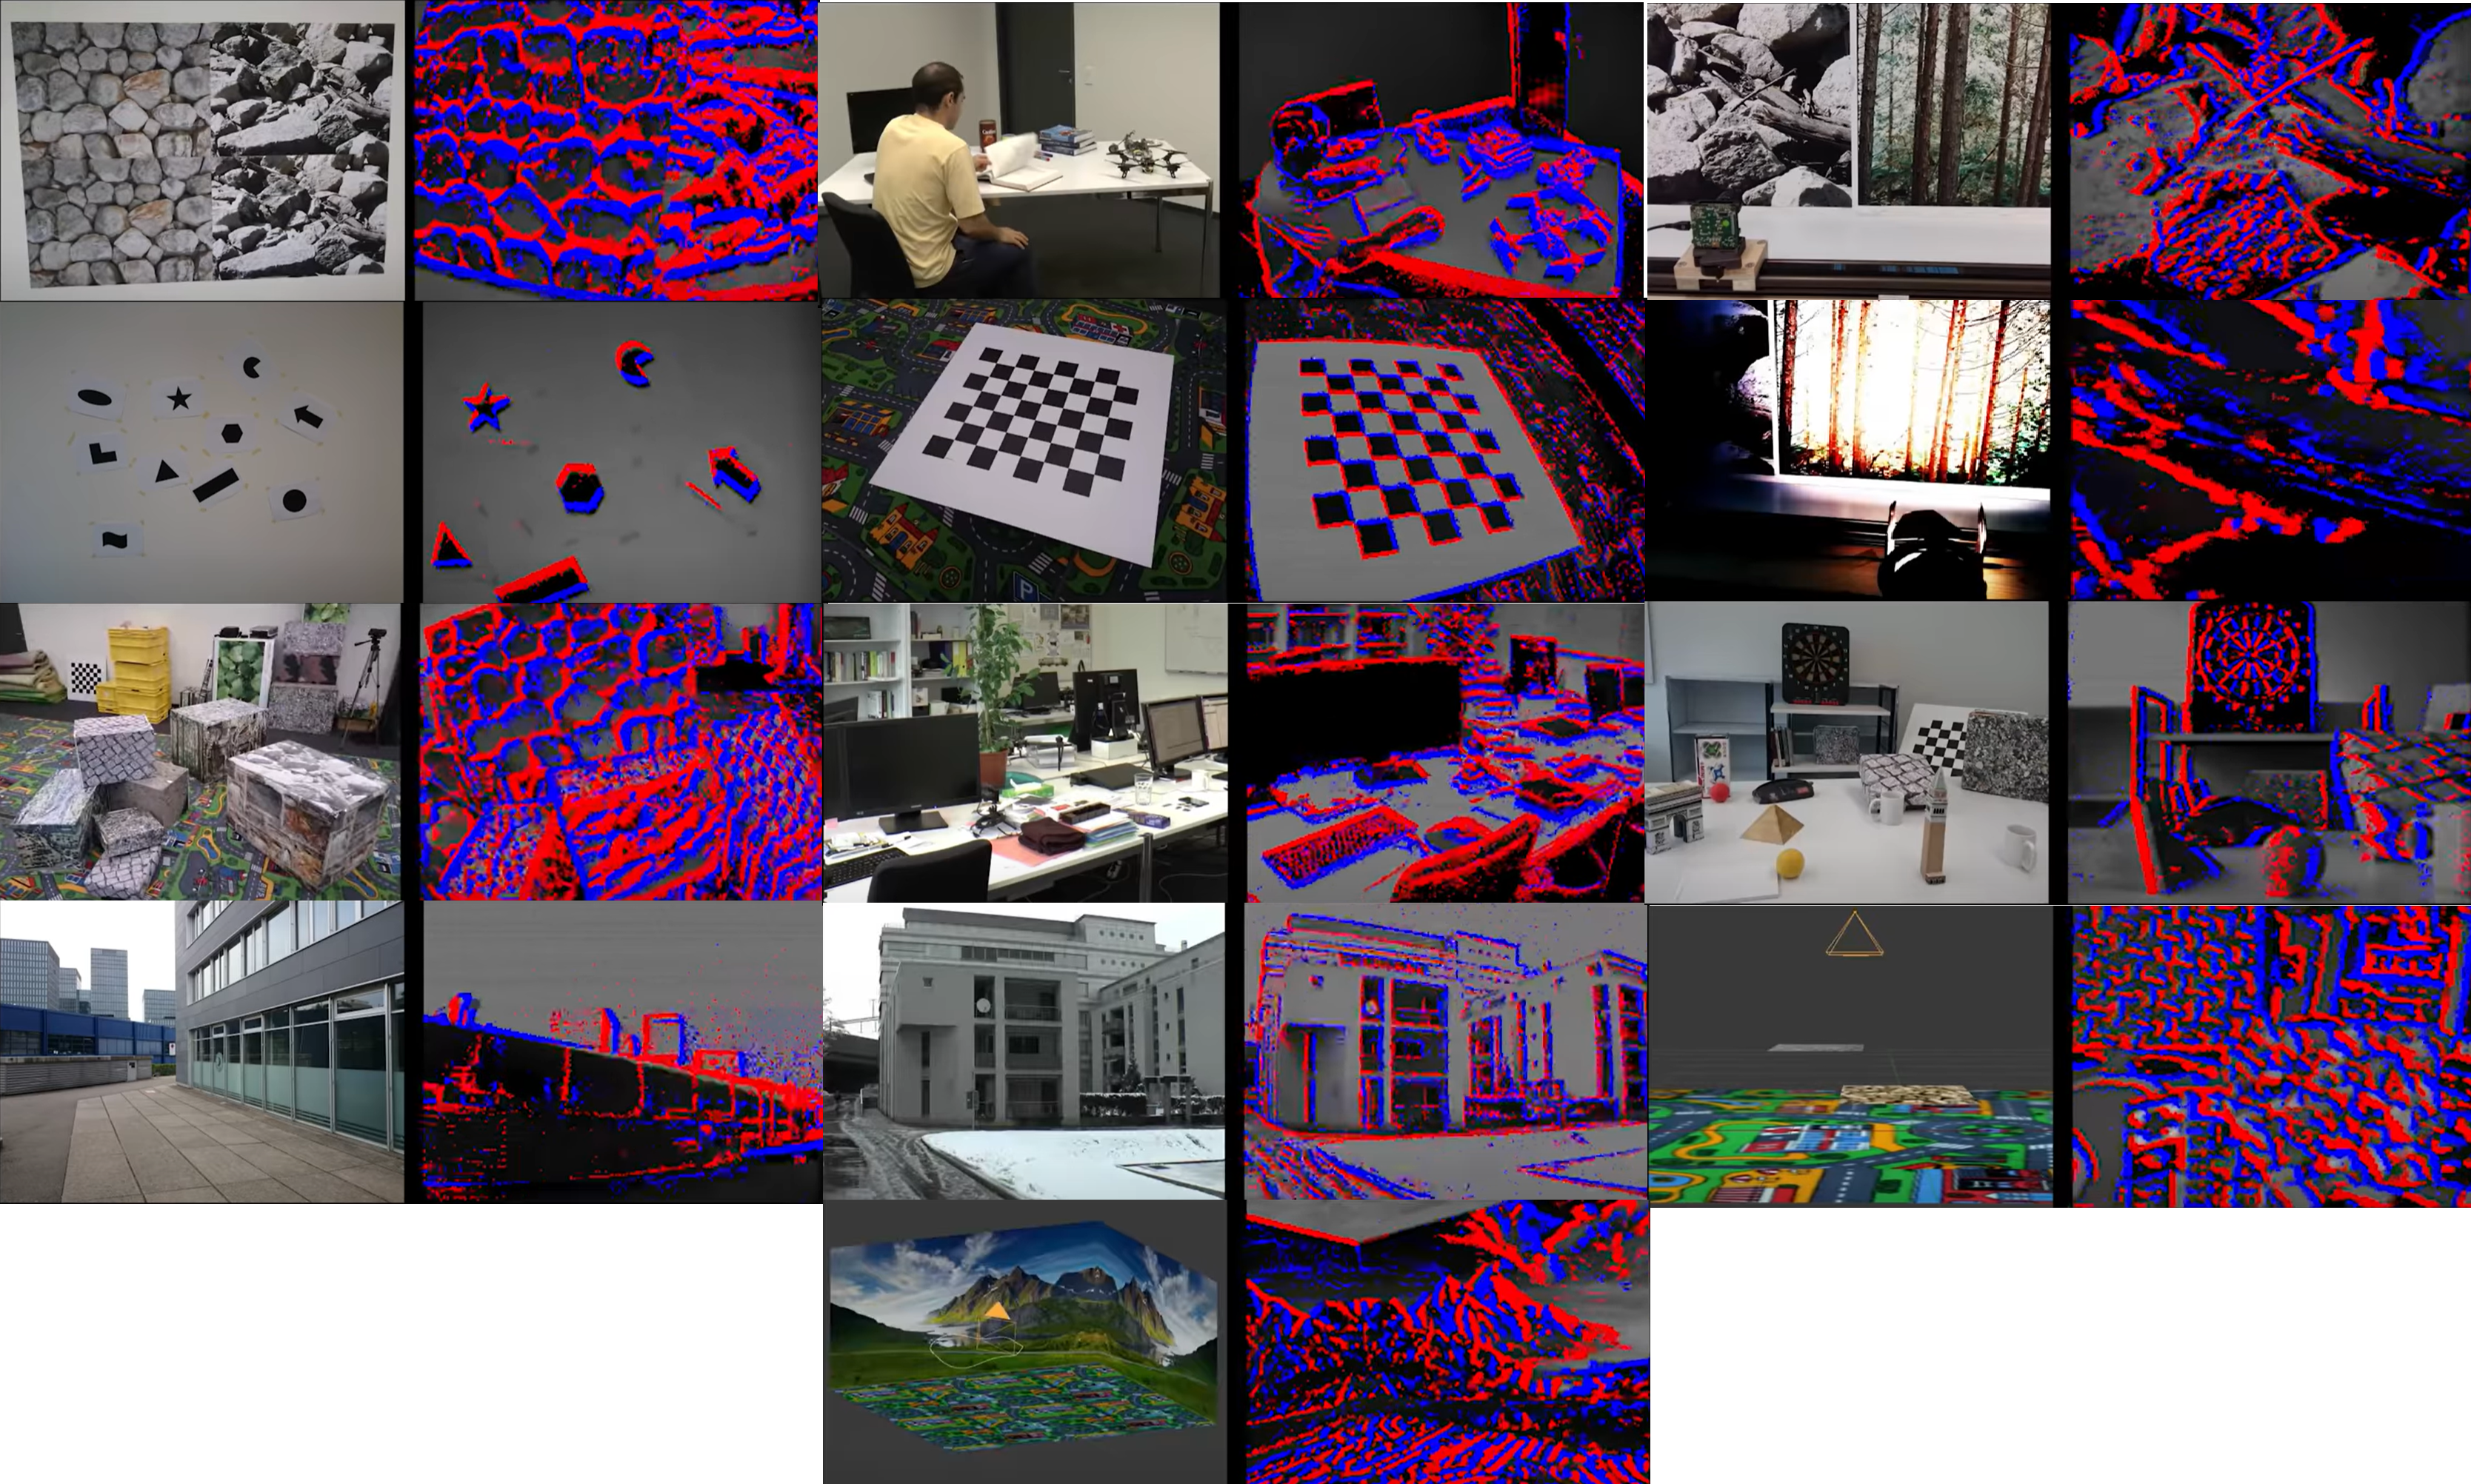
\includegraphics[width=0.5\textwidth]{background/images/event_dataset_videos.png}
      \caption{Visualisation of all videos and events captured in the Event-Camera dataset\cite{EventCameraDataset}.}
      \label{fig:event_dataset_videos}
\end{figure}

\subsubsection{Heridelberg Spiking Datasets} \label{sssec:heridelberg_spiking}

The Spiking Heidelberg datasets for spiking neural networks\cite{SpikingHeidelberg} are useful for realising that spiking data is useful for so many more applications than computer vision. This dataset is split into two; The Spiking Heidelberg Digits (SHD) dataset and the Spiking Speech Command (SSC) dataset. Both of these datasets are audio-based classification datasets for which input spikes and output labels are provided.

\subsection{Non-neuromorphic Datasets}

Other data-sets such as fashion-MNIST could also be converted to spiking times by treating image intensities as input currents to model neurons, so that higher intensity pixels would lead to earlier spikes, and lower intensity to later spikes, as was done by Nicolas Perez-Nieves \textit{et al.}\cite{NeuralHetroPromRobLearn}. This avoids having to own an event-based camera to create data (as was done with the NMNIST dataset mentioned in \cref{ssec:neuromorphic_datasets}), which is useful since the cameras are expensive and difficult to get a hold of in general.

\section{Evaluation Metrics} \label{sec:evalutaion_metrics}

The evaluation plan is as given by the typical machine learning pipeline\cite{IntroToML}. \color{red} TODO: Change this to actual used evaluation metrics and check it fits properly in backround \color{black}

For a classification task, when we obtain the results from the test dataset (as shown in \cref{tab:possible_results}) we can calculate a variety of evaluation metrics that give various insights on our final model.

\begin{table}[htb]
    \centering
    \begin{tabular}{|| c  | c ||}
        \hline
        Labels     & Predictions \\
        \hline \hline
        1          & 1           \\
        \hline
        1          & 2           \\
        \hline
        3          & 8           \\
        \hline
        9          & 9           \\
        \hline
        6          & 9           \\
        \hline
        $ \vdots $ & $ \vdots $  \\
    \end{tabular}
    \caption{A table showing an example of results when inputting test data from NMNIST dataset\cite{NMNIST} into the final model.}
    \label{tab:possible_results}
\end{table}

\subsection{Confusion matrix}

Confusion matrices act as a visualisation of a systems performance. It shows possible true labels as well as possible predicted labels on either side, and filled in are the number of results that fit in each segment. In \cref{tab:confusion_matrix} the confusion matrix for the NMNIST dataset is shown as an example. It should be noted that a similar confusion matrix should be created taking each class as positive, then each metric can be calculated by taking the averages (as shown in \cref{ssec:eval_metric_averaging}). For each of the cells the number of matching records are stored to calculate each of the evaluation metrics. The table includes True Positives (TP), False Positives (FP), True Negatives (TN) and False Negatives (FN).

\begin{table}[htb]
    \centering
    \begin{tabular}{|| c c | c | c | c | c ||}
        \hline
                                                                         &                                    & \multicolumn{4}{ c ||}{\textbf{Predicted Class}}                                        \\
        \cline{3-6}
                                                                         &                                    & 1                                                & 2          & 3          & $ \hdots $ \\
        \hline
        \multirow{6}{*}{\rotatebox[origin=c]{90}{\textbf{Actual Class}}} & \multicolumn{1}{| c |}{1}          & TP                                               & FN         & FN         & $ \hdots $ \\
        \cline{2-6}
                                                                         & \multicolumn{1}{| c |}{2}          & FP                                               & TN         & TN         & $ \hdots $ \\
        \cline{2-6}
                                                                         & \multicolumn{1}{| c |}{3}          & FP                                               & TN         & TN         & $ \hdots $ \\
        \cline{2-6}
                                                                         & \multicolumn{1}{| c |}{4}          & FP                                               & TN         & TN         & $ \hdots $ \\
        \cline{2-6}
                                                                         & \multicolumn{1}{| c |}{5}          & FP                                               & TN         & TN         & $ \hdots $ \\
        \cline{2-6}
                                                                         & \multicolumn{1}{| c |}{$ \vdots $} & $ \vdots $                                       & $ \vdots $ & $ \vdots $ & $ \ddots $ \\
    \end{tabular}
    \caption{a table showing one particular confusion matrix for NMNIST dataset\cite{NMNIST} for class 1 as the positive class.}
    \label{tab:confusion_matrix}
\end{table}

\subsection{Accuracy}

The accuracy of the system is the proportion of samples correctly classified.

$$ Accuracy = \frac{TP + TN}{TP + TN + FP + FN} $$

Note: classification error can also be used and is defined as $ 1 - accuracy $.

\subsection{Precision}

Precision is the proportion of positively predicted samples identified correctly.

$$ Precision = \frac{TP}{TP + FP} $$

It should be noted that a high precision may mean that there are many false positives.

\subsection{Recall}

Recall is the proportion of actual positives correctly classified.

$$ Recall = \frac{TP}{TP + FN} $$

It should be noted that a high recall may mean a lot of positive samples may be missed.

\subsection{F-measure/F-score}

This is defined as the harmonic mean of precision and recall in order to get one number as an average measure of performance.

$$ F_1 = \frac{2 \cdot precision \cdot recall}{precision + recall} $$

\subsection{Micro and Macro Averaging} \label{ssec:eval_metric_averaging}

Macro-averaging involves taking an average on the class level. Metrics are calculated for each class and then averaged at the end. Micro-averaging involves taking an average on the item level (i.e., taking the average of each of TP, FP, TN and FN to get the averages metrics).